
%(BEGIN_QUESTION)
% Copyright 2009, Tony R. Kuphaldt, released under the Creative Commons Attribution License (v 1.0)
% This means you may do almost anything with this work of mine, so long as you give me proper credit

Calculate the two distances ($x_1$ and $x_2$) in this radar level measurement application given echo times of 9.7 ns and 85.3 ns, respectively:

$$\includegraphics[width=15.5cm]{i04219x01.eps}$$

$t_1$ = 9.7 ns

\vskip 10pt

$t_2$ = 85.3 ns

\vskip 10pt

\underbar{file i04219}
%(END_QUESTION)





%(BEGIN_ANSWER)

$x_1$ = 1.328 m

\vskip 10pt

$x_2$ = 4.630 m

%(END_ANSWER)





%(BEGIN_NOTES)


%INDEX% Measurement, interface level: radar

%(END_NOTES)


